
\subsection{Theory}
The contact forces are calculated from creep in the contact plane.
The creep is defined as 
\begin{align}
 \xi_x    &= \frac{V_{wheel,x}}{V_0}\\
 \xi_\eta &= \frac{V_{wheel,\eta}}{V_0}
\end{align}
where $x$ is in the longitudinal direction, $\eta$ is perpendicular $x$ and the normal at the contact point and $V_0$ is the forward velocity of the train.

%Is it the purpose of these derivitions to not assume small deflections, as it is already solved as a nonlinear force.
\begin{figure}[htpb!]
 \centering
  \includegraphics[width=0.8\textwidth]{figures/QQ_0409.pdf}
 \caption{A plot!}
 \label{fig:plot} % Labels must come after caption!
\end{figure}

\begin{figure}[htpb!]
\centering
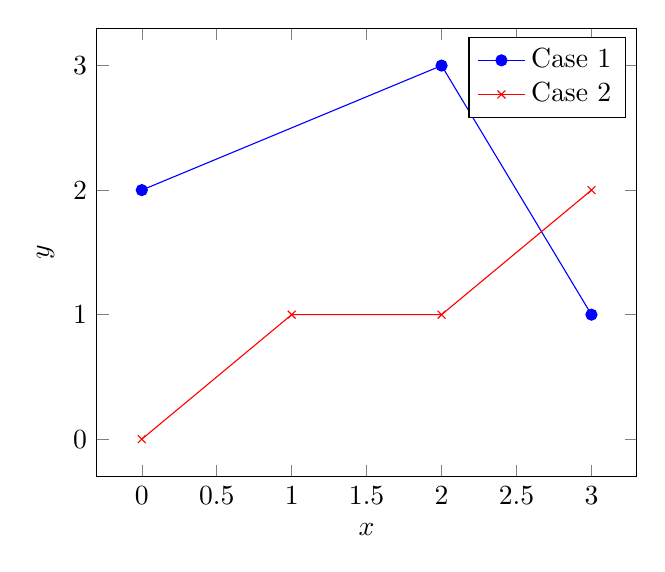
\begin{tikzpicture}
  \begin{axis}[xlabel=$x$,ylabel=$y$]
   \addplot[color=blue,mark=*] plot coordinates { (0,2) (2,3) (3,1) };
   \addlegendentry{Case 1}
   \addplot[color=red,mark=x] plot coordinates { (0,0) (1,1) (2,1) (3,2) };
   \addlegendentry{Case 2}
  \end{axis}
 \end{tikzpicture}
 \caption{A tikz plot!}
 \label{fig:tikz_plot}
\end{figure}

Right side refers to the right in the forward direction of the train, i.e. the right wheel is not shown in figure \ref{fig:plot}.

The velocities can now be calculated as
% \begin{align}
% \omega_0 &= \frac{V_0}{r_0}\\
%  s       &= \begin{cases}+1&\text{if right side}\\-1&\text{if left side}\end{cases}\\
%  r       &= r[-s x_2]\\
%  w       &= s w_0 - x_2\\
%  \uv{d}  &= \begin{pmatrix}0\\w\\r\end{pmatrix}\\
%  \um{R}_z     &= \begin{pmatrix}
%         \cos[-\varphi_3] & -\sin[-\varphi_3] & 0\\
%         \sin[-\varphi_3] &  \cos[-\varphi_3] & 0\\
%         0                &  0                & 1
%      	\end{pmatrix} \\
%  \uv{V}_{wheel} &= \uv{\dot{x}} +\begin{pmatrix}V_0\\0\\0\end{pmatrix} + \um{R}_z \cdot (\uv{d} \times (\uv{\dot{\varphi}}+\begin{pmatrix}0\\\omega_0\\0\end{pmatrix}))
% \end{align}
where the $r$ is an interpolating function of the geometry of a standardized S1002 wheel profile \cite{railvehicledynamics_eandersson}.

\begin{table}[htpb!]
 \centering
 \caption{Explanation of variables for calculating the creep.}
 \begin{tabular}{c | l}
  $\uv{x}$       & Translation vector of wheelset.\\
  $\uv{\varphi}$ & Rotation vector of wheelset.\\
  $r_0$		 & Wheel radius at nominal contact point.\\
  $r$            & Wheel radius at current contact point.\\
  $w_0$		 & Lateral distance from COG to nominal contact point.\\
  $w$		 & Lateral distance from COG to current contact point.\\
  $V_0$		 & Nominal forward velocity of train.\\
  $\omega_0$	 & Nominal angular velocity of wheels.\\
  $\delta$	 & Inclination of wheels (positive).\\
  $s$		 & Side dependence, +1 for right side, -1 for left side.
 \end{tabular}
\end{table}

\subsubsection{Contact Patch Dimensions}
To calculate the forces the dimensions of the contact patch are required.
According to Hertz theory the dimensions are calculated as \cite{hallfasthetslara_bsundstrom} and \cite{railvehicledynamics_eandersson}
\begin{align}
 A+B    =& \frac12 \left(\frac{1}{r_{\eta,r}}+\frac{1}{r_{\eta,w}}+\frac{1}{r_{x,r}}+\frac{1}{r_{x,w}} \right)\\
 \nonumber B-A =& \frac12 \left(\left(\frac{1}{r_{x,r}}-\frac{1}{r_{\eta,r}}\right)^2 + 
                          \left(\frac{1}{r_{x,w}}-\frac{1}{r_{\eta,w}}\right)^2 +\right.\\
               &\left.   2\left(\frac{1}{r_{x,r}}-\frac{1}{r_{\eta,r}}\right)
                          \left(\frac{1}{r_{x,w}}-\frac{1}{r_{\eta,w}}\right)\cos[2\phi_z]\right)^\frac12\\
 \Psi   =& \sqrt[3]{\frac{3 N}{2 (A+B)} \left(\frac{1-\nu_w^2}{E_w} +\frac{1-\nu_r^2}{E_r}\right)}\\ 
 \theta =& \arccos\left[\frac{B-A}{A+B}\right]\\
 a      =& m \Psi\\
 b      =& n \Psi
\end{align}
where $m = m[\theta]$ and $n = n[\theta]$. There is no explicit expression for $m[\theta]$ or $n[\theta]$ but they can be solved numerically with (4.25) through (4.32) in \cite{contact_mechanics_kljohnson}. This has been done in table 8-1 in \cite{railvehicledynamics_eandersson} which values are used.

\begin{table}[htpb!]
 \centering
 \caption{Explanation of variables for calculating the creep.}
 \begin{tabular}{c | l}
  $N$                                     & Normal force in contact.\\
  $E_w,E_r$                               & Modulus of elasticity in the wheel and rail.\\
  $\nu_w,\nu_r$                           & Poissons ratio for the wheel and rail.\\
  $a,b$                                   & Contact patch dimension along $x$ and $\eta$.\\
  $r_{x,w},r_{x,r},r_{\eta,w},r_{\eta,r}$ & Radius around the respective axis for wheel and rail.\\
  $\phi_z$                                & The angle of the wheel.
 \end{tabular}
\end{table}
The radius $r_{\eta,r}$ is zero since the rail is straight. 
The other radii varies with the contact point and wheel profile. However they are approximated as constant for the contact geometry at a point far from the flange where the wheel is almost flat. In that case $r_{x,w}=\infty$ and $r_{\eta,w} = r$.
For the wheel the radius over the top of the rail is almost constant and be approximated as $r_{x,r} = 300$mm.
In this case $\eta$-axis is parallell with the $y$-axis.
The effect from the rotation of the wheel is also neglected, as this angle will always be small, i.e. linearisation of $cos[2\phi_z] \approx 1$. This simplifies the equations and with the approximations of the radii the variables $m$ and $n$ are constant.

The rest of the material parameters were set to $E_w = E_r = 200$ GPa and $\nu_w = \nu_r = 0.3$.

\subsubsection{Wheel Forces from Creep}
The creep forces are calculated with Kalker's linear theory \cite{railvehicledynamics_eandersson}.
The coefficients for the creep, $\uv{C} = \uv{C}[\frac{a}{b}]$, are interpolated from a set of data taken from table 8-2 in \cite{railvehicledynamics_eandersson}.

\begin{align}
 \uv{F}_{lin} &= - G a b \begin{pmatrix}
                          C_{11} \xi_x\\C_{22} \xi_\eta
                         \end{pmatrix}\\
 u            &= \frac{|\uv{F}_{lin}|}{\mu N}\\
 \uv{\hat{F}} &= \uv{F}_{lin} \begin{cases}
                  1-\frac{u}{3}+\frac{u^2}{27} &\text{if $u < 3$} \\
                  \frac{\mu N }{|\uv{F}_{lin}|} & \text{otherwise}
                 \end{cases}
\end{align}

The behaviour of the flange will be greatly simplified as done in \cite{appwheelrailcurvedtracks_jpombo}
\begin{align}
 F_{flange} = \begin{cases}
               k_{flange}( n_{flange}-x_2) & \text{if } x_2 >  n_{flange} \wedge s > 0 \text{ (right side)}\\
               k_{flange}(-n_{flange}-x_2) & \text{if } x_2 < -n_{flange} \wedge s < 0 \text{ (left side)}\\
               0                           & \text{otherwise}
              \end{cases}
\end{align}
where $F_{flange}$ acts in the $y$-axis and is added to  $F_y$.

The force vector $\uv{\hat{F}}$ is here acting on the contact plane, so to get the horizontal component
\begin{align}
 \uv{F} = \begin{pmatrix}
           F_x\\
           F_y
          \end{pmatrix} =
          \begin{pmatrix}
           \hat{F}_1\\
           \hat{F}_2\frac{\delta}{\sqrt{1+\delta^2}}+F_{flange}
          \end{pmatrix}
\end{align}

The contributions to the nonlinear force on the system will be
\begin{align}
 \uv{R}_e = \begin{pmatrix}
      F_x\\F_y\\0\\ 0\\r F_x\\-w F_x -w F_y \sin[\phi_3]
     \end{pmatrix}
\end{align}
which is assembled into $\uv{R}$ for each wheel.
